% !TeX root = ../main.tex

\chapter{影像分析 Agent：模型微调与推理}
\label{sec:image-analysis-agent}

本项目在模型层面的设计目标，并不是简单完成牙科影像的目标检测，而是在通用视觉语言模型的基础上，构建一个能够适配口腔场景的多模态专用模型，使其既能识别牙科影像中的关键目标，又能够以中文完成结构化描述、结果摘要和后续问答推理。基于这一目标，项目整体采用“通用多模态基座+领域指令数据+分阶段 LoRA 微调+本地推理部署”的技术路线。影像分析 Agent 正是该技术路线在 OralSage 系统中的工程封装：前端负责影像上传与结果展示，后端负责多模态请求构造与模型服务调用，OralPath-VL 视觉模型负责完成口腔影像理解与结构化输出。

\section{微调数据集}

本项目在模型适配部分主要使用团队自行整理的专门针对牙科疾病诊断设计的高精度多模态数据集。该数据集涵盖了 31 类口腔病理特征、治疗状态及解剖结构。

该数据集共包含 31 类牙科结构与病变目标，覆盖 4 大口腔临床领域，如表~\ref{tab:oralpath-target-overview} 所示。

\begin{table}[H]
  \centering
  \caption{牙科结构与病变目标概述}
  \label{tab:oralpath-target-overview}
  \small
  \renewcommand{\arraystretch}{1.18}
  \begin{tabularx}{\linewidth}{p{0.20\linewidth}X}
    \toprule
    领域 & 类别 \\
    \midrule
    牙体牙髓 & Caries（龋坏）、Filling（充填）、Root Canal Treatment、Periapical lesion、Root resorption、Fracture teeth \\
    修复/种植 & Crown（牙冠）、Implant（种植体）、Abutment、Post-core、Retained root、Root Piece \\
    牙周/颌骨 & Bone Loss、Bone defect、Cyst（囊肿）、Maxillary sinus、Mandibular Canal \\
    正畸/其他 & Orthodontic brackets、Wire、Metal band、TAD、Permanent retainer、Malaligned、Missing teeth、Supra Eruption 等 \\
    \bottomrule
  \end{tabularx}
\end{table}

经过前述处理方案后，本项目团队获得了三类基础任务数据：

1、结构化定位任务，用于训练模型识别图中目标并输出标准化的 JSON 结果；

2、中文摘要任务，用于训练模型根据牙科影像中的已标注信息生成较符合临床表达习惯的中文摘要；

3、长尾类别聚焦任务，用于针对低频类别进行专项补强。最终，这些数据又被统一整合为混合型训练数据集，用于后续多任务联合训练。

\begin{figure}[H]
  \centering
  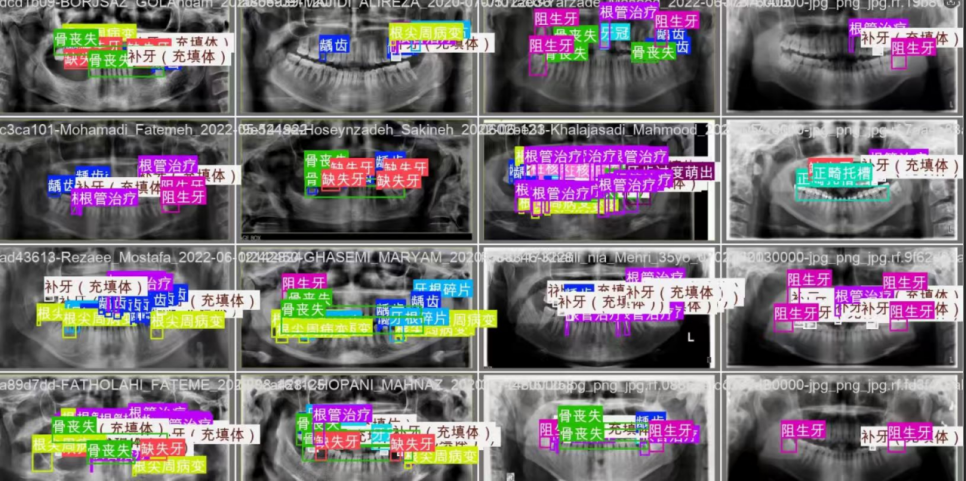
\includegraphics[width=0.96\linewidth]{oralpath-fig17-multimodal-data.png}
  \caption{高精度多模态数据部分示意}
  \label{fig:oralpath-multimodal-data}
\end{figure}

根据上述数据集的特性与 OralSage 项目的定位，本项目设计了如下模型微调方案，使模型在保持通用能力的同时具备更强的口腔专业理解能力。

\section{基座模型}

本项目采用“通用大模型推理 + 专科小模型微调”的组合架构。

在 Agent 实际运行中，调用 Pro/Qwen/Qwen2.5-7B-Instruct 处理纯文本逻辑，调用 volcano 处理语音交互，从而保证日常对话、文本理解和语音输入输出具有较好的稳定性与响应速度；而在口腔影像识别、多模态理解和图文联合推理等核心任务上，项目团队并未直接依赖通用模型，而是单独选择一套适合作为领域微调基座的视觉语言模型，用于构建面向口腔场景的专用多模态能力。

结合项目的实际需求与运行环境，本项目最终选取 Qwen/Qwen2.5-VL-7B-Instruct 作为微调基座模型。其选择并非单纯因为参数规模适中，而是综合考虑了口腔影像的图像特点、多模态任务形式、以及后续本地部署的可行性。从整体原则上看，本项目的模型选型主要围绕四个关键词展开：适配口腔影像特点、支持多模态推理、能够稳定调用，以及具备较好的轻量化与工程部署能力。

1、视觉感知适配性：面向口腔特殊影像结构

口腔全景片（OPG）具有“幅面宽、细节密”的特点。若使用常规 VLM，往往需要对图像进行填充（Padding）或拉伸，导致无效计算或特征变形。本项目利用 Qwen2.5-VL 的 M-RoPE（旋转位置编码）机制，将全景片切分为多个 Patch 进行序列化输入，在不增加显存开销的前提下，实现了对全景片原始分辨率的完整保留。

2、多模态推理一致性：支持图文联合决策场景

口腔诊疗决策是典型的多模态任务（X 光 + 主诉 + 既往史）。Qwen2.5-VL 支持图像与长文本的交错输入（Interleaved Input），使得系统可以将“患者全景片”与“RAG 召回的文本指南”作为一个完整的 Prompt 输入给模型。这种设计避免了传统“视觉模型看图 + 语言模型看文”的分离式架构带来的语义损耗，显著提升了解释型回答（Explainable AI）的准确性。

3、模型规模与成本平衡：兼顾效果与训练部署效率

对于口腔领域这样的垂直场景，项目目标不是训练一个超大规模通用模型，而是在有限的时间和算力约束下，构建一个“足够强、且可部署”的专科视觉语言模型。如果选择更大规模的多模态模型，虽然可能在通用任务上有更强的上限，但训练成本、显存占用、推理时延以及后续部署复杂度都会明显提升，不利于项目在竞赛场景与实际平台中的快速落地。而 7B 级别模型在当前硬件环境下已经能够较好地支撑 LoRA 微调、本地测试和后续服务封装，同时在效果与效率之间取得较合理平衡。

4、工程接入可行性：适配本地服务链路

Qwen2.5-VL 作为当前社区中兼容性较好、生态较成熟的视觉语言模型，在本地推理服务构建、LoRA 微调适配、模型权重导出以及 OpenAI-compatible 接口封装方面都具有较好的工程基础，这使得项目团队可以在较短时间内打通“模型训练—模型评测—模型部署—平台接入”的闭环，而不必将大量精力消耗在底层兼容问题上。

\begin{figure}[H]
  \centering
  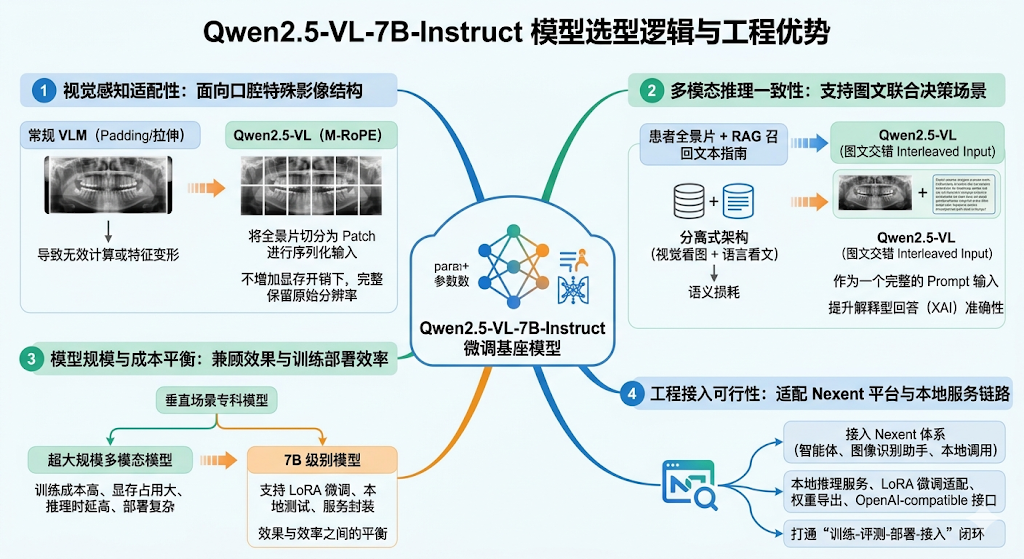
\includegraphics[width=0.96\linewidth]{oralpath-fig18-qwen-vl-design.png}
  \caption{Qwen2-VL-7B 模型微调设计思路}
  \label{fig:oralpath-qwen-vl-design}
\end{figure}

基于上述特性，项目团队采用 Qwen/Qwen2.5-VL-7B-Instruct 的微调版本作为“口腔多模态能力”的核心支撑模型。在此基础上，再利用口腔领域图像数据和转换后的多模态指令数据进行 LoRA 微调，使模型逐步获得面向牙科影像的目标识别、结构化定位、中文摘要表达和长尾类别补强能力。

从实际项目需求来看，本研究并不打算重新训练一个全新的牙科多模态模型，而是希望在高质量通用模型基础上，利用专科领域数据进行适配，使模型逐步获得口腔影像理解能力。采用 Qwen2.5-VL-7B-Instruct 作为基座，可以保留通用视觉语言推理能力，并通过较低成本的领域微调，使其更适合口腔场景中的图像理解与问答需求。

\section{设计思路概述}

模型微调的整体思路可以概括为“先建立主体能力，再补强薄弱类别，最后衔接推理和评测”。在训练逻辑上，项目并未采用单轮单任务微调方式，而是根据口腔场景的实际需求，将训练过程设计为分阶段的领域适配过程。

1、第一阶段：主训练阶段

该阶段使用混合型多任务数据集，让模型同时学习目标识别、位置表达和中文摘要能力。这样做的目的，是让模型优先建立对口腔影像中“主要对象”和“主要表达方式”的整体理解，而不是只停留在单一检测任务上。

2、第二阶段：长尾类别补强阶段

由于原始牙科数据中不同类别之间分布极不均衡，部分重要病变和器械类别样本数量很少，如果不单独强化，模型容易在高频类别上表现良好，却对稀有类别缺乏敏感性。因此，在主训练完成后，项目再使用长尾类别聚焦数据集对模型进行二次补强。

3、第三阶段：推理评测阶段

在微调完成后，通过快速评测和全量评测两种方式，对模型在测试集上的表现进行验证，并为后续本地部署和智能体调用提供依据。

\begin{figure}[H]
  \centering
  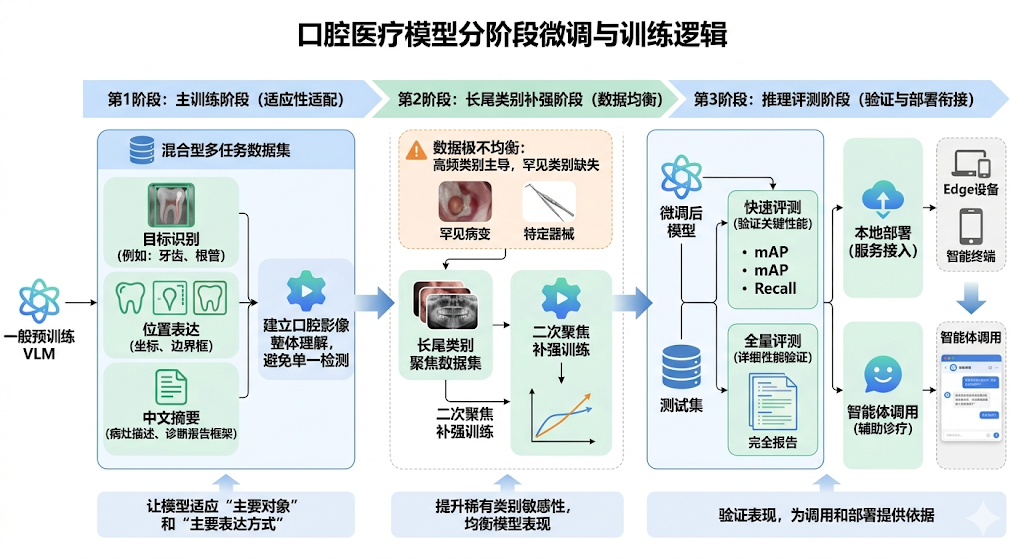
\includegraphics[width=0.96\linewidth]{oralpath-fig19-training-logic.png}
  \caption{口腔医疗模型微调与训练逻辑}
  \label{fig:oralpath-training-logic}
\end{figure}

这种设计的核心思想，是把“会识别”“会描述”和“会关注难例”拆分成相互衔接的训练目标，而不是试图在一次训练中同时解决所有问题。这样既能提升训练效率，也能使每个阶段的目标更加清晰。

\section{详细微调策略}

针对口腔医疗场景中影像长宽比特殊（全景片）、病灶细微（如早期龋齿）、专业术语复杂等挑战，本项目并不是沿用传统“单一任务、单轮训练”的方式，而是围绕口腔影像场景的特点，构建了一套面向视觉语言模型的多任务、分阶段、渐进式领域适配方案：

\subsection{训练目标}

本项目没有将微调任务限制为单一的目标检测式输出，而是将原始牙科影像标注扩展为多个层次的视觉语言学习任务。模型既需要学习“图像中有哪些目标、它们位于何处”，又需要学习“如何将这些目标组织成符合口腔场景的中文描述”，同时还需要在样本极不均衡的前提下，尽可能保留对稀有类别的识别能力。

基于这一考虑，项目将整个微调目标划分为三个互补方向：其一是结构化定位学习，其二是中文摘要表达学习，其三是长尾类别强化学习。三者并不是相互割裂的独立任务，而是在同一模型内部共同推动口腔领域能力的形成。

\subsection{训练流程安排}

在训练流程安排上，本项目采用了分阶段渐进式微调策略。

第一阶段为主体能力建立阶段，其任务重点在于让模型完成对口腔影像主要目标的识别与理解，并初步掌握中文描述方式。这一阶段并不刻意追求对所有细小类别的极致表现，而是优先建立稳定的领域基础能力，使模型先学会“看懂图像、说清结果”。

第二阶段为长尾类别补强阶段，其任务重点不再是全面学习，而是将有限训练资源集中到样本较少、但临床意义较强的类别上。

通过这种“先整体、后细节”的训练安排，可以避免模型在一开始就被复杂的类别长尾分布打乱训练节奏，同时也能够减少高频类别对低频类别的梯度压制问题。

\begin{figure}[H]
  \centering
  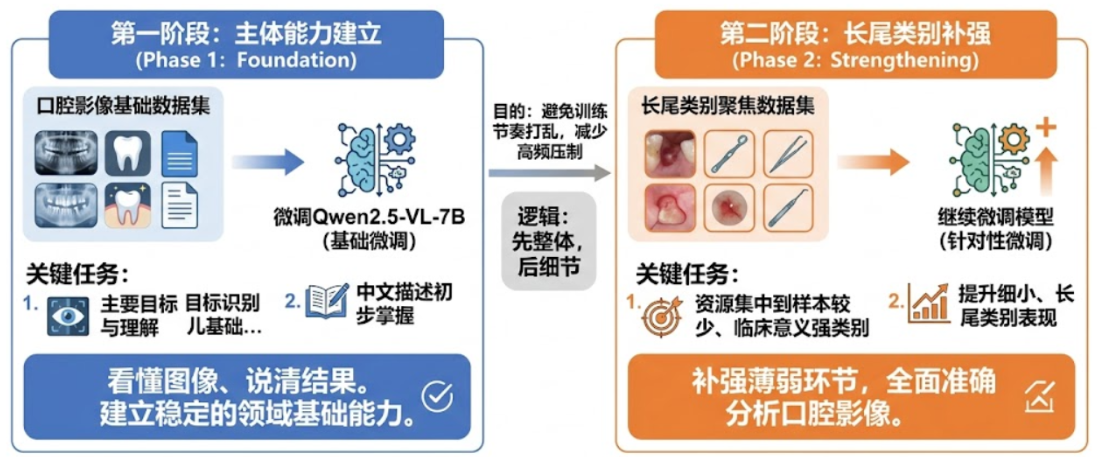
\includegraphics[width=0.96\linewidth]{oralpath-fig20-training-flow.png}
  \caption{训练流程安排}
  \label{fig:oralpath-training-flow}
\end{figure}

\subsection{具体训练方案}

在具体训练方法上，本项目采用的是 LoRA（Low-Rank Adaptation）参数高效微调方案。

相比全参数训练，LoRA 不需要对整个大模型的全部参数进行更新，而是仅在核心线性层中引入少量可训练参数，从而在尽量保留基座模型原有通用能力的同时，快速完成口腔领域知识与视觉特征的适配。

之所以采用 LoRA 而非全参数微调，一方面是考虑到多模态大模型训练成本高、工程复杂度大，另一方面也是希望在不破坏通用图文推理能力的前提下，让模型获得更稳定、更可控的专科迁移效果。LoRA 方案在训练效率、显存占用、模型可复用性以及最终权重导出方面都具有明显优势。

\begin{figure}[H]
  \centering
  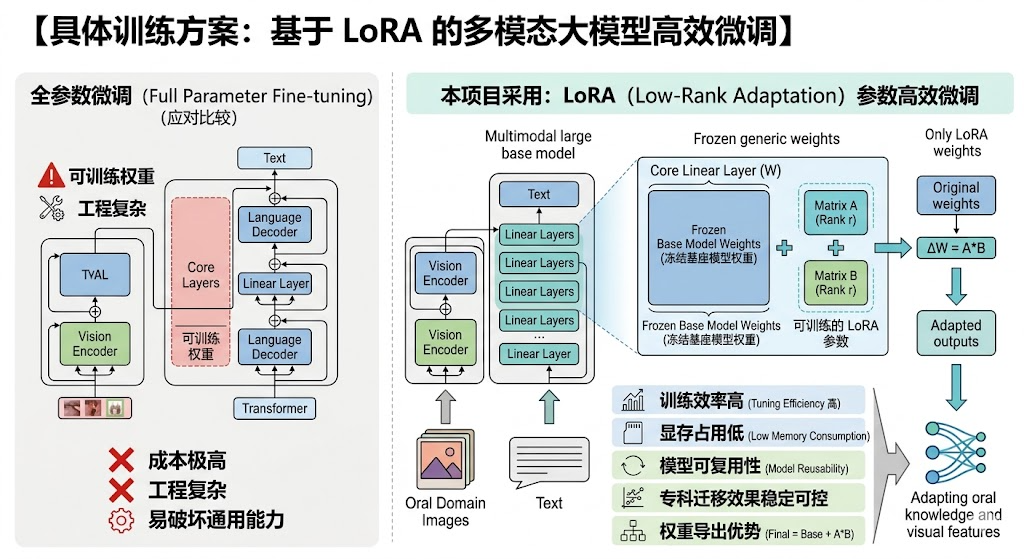
\includegraphics[width=0.96\linewidth]{oralpath-fig21-lora-scheme.png}
  \caption{基于 LoRA 的多模态大模型微调方案}
  \label{fig:oralpath-lora-scheme}
\end{figure}

\subsection{训练执行细节}

在训练执行细节上，本项目进一步结合当前硬件条件与模型特性，采用了一组面向稳定性和效率优化的训练策略。

1、混合精度计算：以降低显存占用并提高吞吐效率；

2、梯度检查点机制，以在不显著损失模型表达能力的前提下缓解长序列图文输入带来的显存压力。

3、优化器选择：优先采用 fused 版本的 AdamW，以提高训练阶段的实际执行效率。

4、输入控制：根据不同阶段任务的特点对输入长度进行区分设置：

（1）主体训练阶段保留更充分的图文上下文，确保模型能够同时处理定位信息和中文摘要信息；

（2）长尾补强阶段则适当压缩输入长度，使模型更专注于长尾类别本身，从而在有限时间内提升专项学习效率。

\subsection{创新性微调策略说明}

（一）面向多任务融合的视觉语言训练框架

本项目微调策略的一个重要创新点，在于并未简单将检测标注数据“翻译”为文本，而是把检测任务、图文摘要任务和长尾聚焦任务共同纳入统一的视觉语言训练框架中。传统检测数据集通常只能训练模型完成目标识别和位置回归，而本项目通过任务重构，使同一份牙科影像数据同时承担“目标定位监督”“中文表达监督”和“长尾类别监督”三类角色。这种设计使模型不再只具备“框出目标”的能力，而能够进一步具备“解释图像中目标及其临床含义”的能力，更符合口腔智能助手的真实使用需求。

（二）面向长尾类别的专项补强训练思路

口腔影像数据天然存在类别分布不均问题，常见修复体和常见牙列结构远多于少见病变和特殊器械。如果只依赖混合训练，模型通常会优先收敛到高频类别，对稀有类别表现不足。

针对这一问题，本项目并未仅依赖重采样或损失加权，而是进一步通过“任务级别聚焦”的方式，让模型在专门的长尾指令中只关注特定类别，从而显式强化低频目标在模型内部的表示能力。这种做法本质上是将类别不平衡问题从“样本分布问题”提升为“任务设计问题”来处理，具有较强的针对性。

（三）“主训练 + 补强训练”的层次化领域适配路径

许多传统领域微调方案会直接使用全部数据进行统一训练，但这种做法在面对复杂多模态任务时，往往容易造成模型在训练早期目标不清、学习方向混杂。本项目将“主体能力构建”和“长尾能力强化”明确拆分为不同阶段，使模型在主训练阶段优先获得稳定的口腔影像识别与表达基础，再在第二阶段补足其对少样本类别的关注能力。这样的安排不仅提高了训练的可解释性，也更有利于控制不同阶段的目标与风险。

\begin{figure}[H]
  \centering
  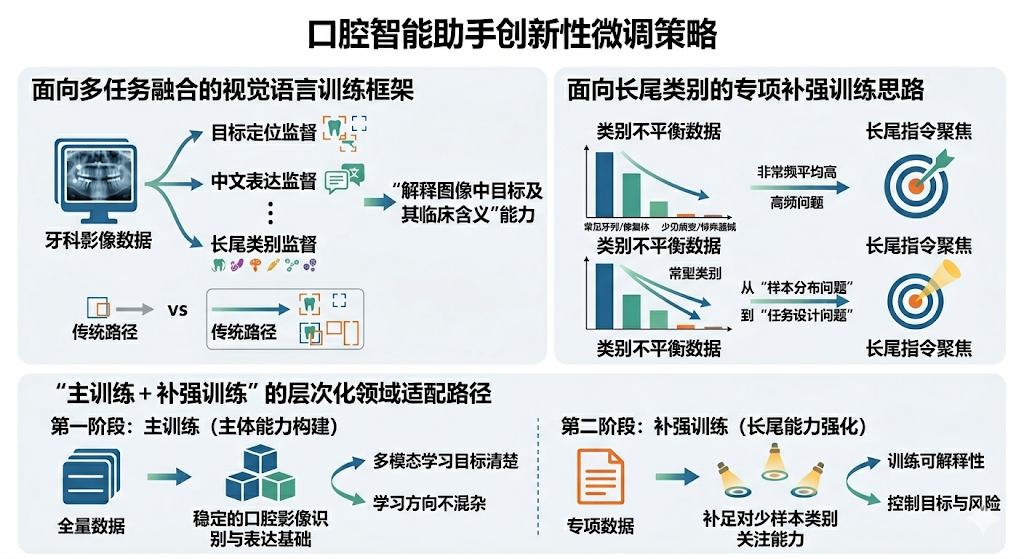
\includegraphics[width=0.96\linewidth]{oralpath-fig22-innovation-strategy.png}
  \caption{创新性微调策略说明}
  \label{fig:oralpath-innovation-strategy}
\end{figure}

总体来看，本项目的详细微调策略可以概括为：以高质量通用视觉语言模型为基座，以口腔影像多任务指令数据为训练核心，以 LoRA 为主要适配方式，以分阶段训练和长尾补强为优化重点，以部署可落地为最终导向。这一策略既兼顾了口腔场景下的识别精度与表达能力，也兼顾了当前实验资源约束、训练周期控制和后续部署实施的现实要求。

\section{微调结果自测及说明}

为验证模型在口腔场景下的实际适配效果，项目团队在主训练完成后，依次对模型进行了训练过程自检、长尾类别补强验证以及多轮快速评测。

考虑到本项目的训练目标并不单一，既包含结构化定位任务，也包含中文摘要任务，因此在结果验证阶段没有仅依赖通用文本相似度指标，而是结合任务特点分别采用了训练损失、验证损失、文本类指标和结构化指标进行综合分析，尽可能从“模型是否稳定收敛”“模型是否具备口腔领域表达能力”“模型是否真正学会结构化识别”三个层面，对当前模型效果作出较全面判断。

\subsection{训练收敛情况}

在训练流程上，模型首先完成了主训练阶段，再完成了长尾类别补强阶段。主训练阶段面向多任务混合数据展开，重点学习口腔影像中的主体目标识别能力和中文摘要表达能力；长尾补强阶段则聚焦于稀有类别，进一步增强模型对少样本病变和器械目标的敏感性。当前训练结果表明，两阶段训练整体过程是稳定的，未出现明显的发散或训练崩溃现象。

主训练阶段共完成 2410 个优化步，最佳验证点出现在 checkpoint-2000，其最佳验证损失为 0.2144，最终训练损失约为 0.2572。

从训练曲线看，损失值整体呈下降趋势，说明模型已经较稳定地完成了从通用多模态基座向口腔场景的主体能力迁移。

长尾补强的第二轮训练共完成 99 个优化步，最佳验证点出现在 checkpoint-50，对应的验证损失约为 0.3955，最终训练损失约为 0.4098。由于长尾补强阶段的数据分布更稀疏、任务目标更聚焦，因此其损失数值不能简单与主训练阶段横向比较，但从训练日志和收敛趋势看，该阶段同样保持了稳定优化，没有出现明显的过拟合失控现象。

\subsection{评测策略说明}

由于本项目的训练数据同时包含结构化定位任务、中文摘要任务和长尾类别聚焦任务，因此单一评测方式很难完整反映模型能力。项目团队在评测阶段采取了“两层评测”的思路。

1、基于文本相似度的快速评测，用于观察模型整体输出是否已经偏离参考答案；

2、面向任务本身的结构化评测，用于更准确判断模型在 JSON 输出、类别识别、目标匹配和中文摘要等方面的真实表现。

其中，结构化评测是当前最值得参考的一组结果。原因在于，检测型任务和长尾聚焦任务本质上都要求模型输出可解析的结构化 JSON，如果只使用 ROUGE 或 Token F1 来评价，容易低估模型在类别和位置上的真实能力，也容易因为字段顺序变化而误判结果。因此，本项目对 detection\_json 和 rare\_focus\_json 任务采用了更贴合任务的指标：包括 JSON 可解析率、结构化完全匹配率、类别识别 F1、目标数量误差、IoU 条件下的检测精度与召回率，以及已命中目标的平均 IoU。同时，对 summary\_zh 任务保留文本相似度指标，用于评估模型的中文摘要表达能力。

\begin{figure}[H]
  \centering
  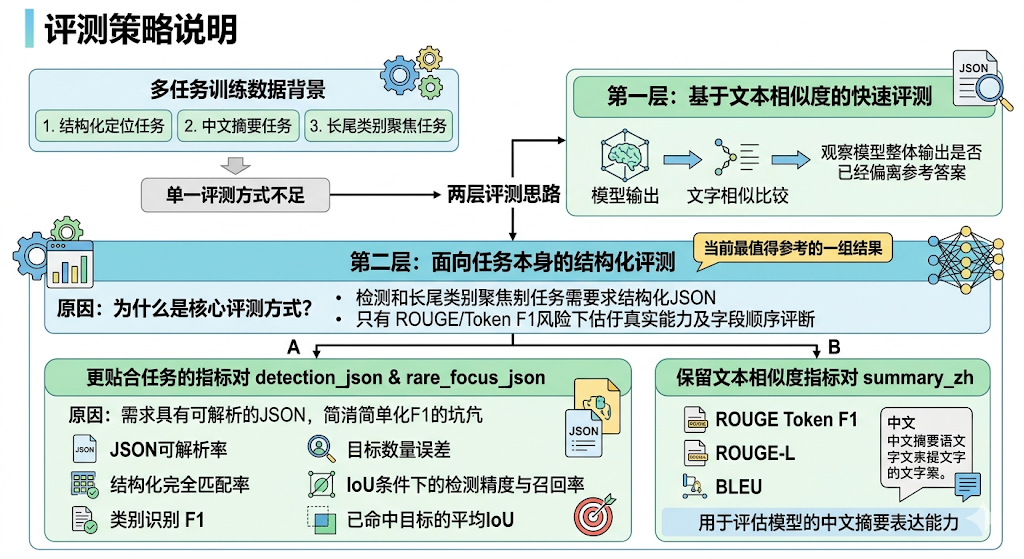
\includegraphics[width=0.96\linewidth]{oralpath-fig23-evaluation-strategy.png}
  \caption{评测策略说明}
  \label{fig:oralpath-evaluation-strategy}
\end{figure}

\subsection{口腔 X 片中文摘要能力评测}

为了验证 OralPath 在口腔影像场景中的实际应用能力，项目团队重点对模型的口腔 X 片中文摘要生成能力进行了专项评测。之所以将这一能力单独抽出进行分析，是因为在口腔临床场景中，医生对于模型的需求并不只是“识别出图中某个目标”，而更希望模型能够对整张影像中的主要发现进行归纳、提炼并用符合医学语义的中文表达出来。

相比单纯的结构化框输出，口腔 X 片摘要能力更接近实际应用中“图像辅助解读”的使用需求，也是 OralPath 当前最具代表性的优势能力之一。

\begin{figure}[H]
  \centering
  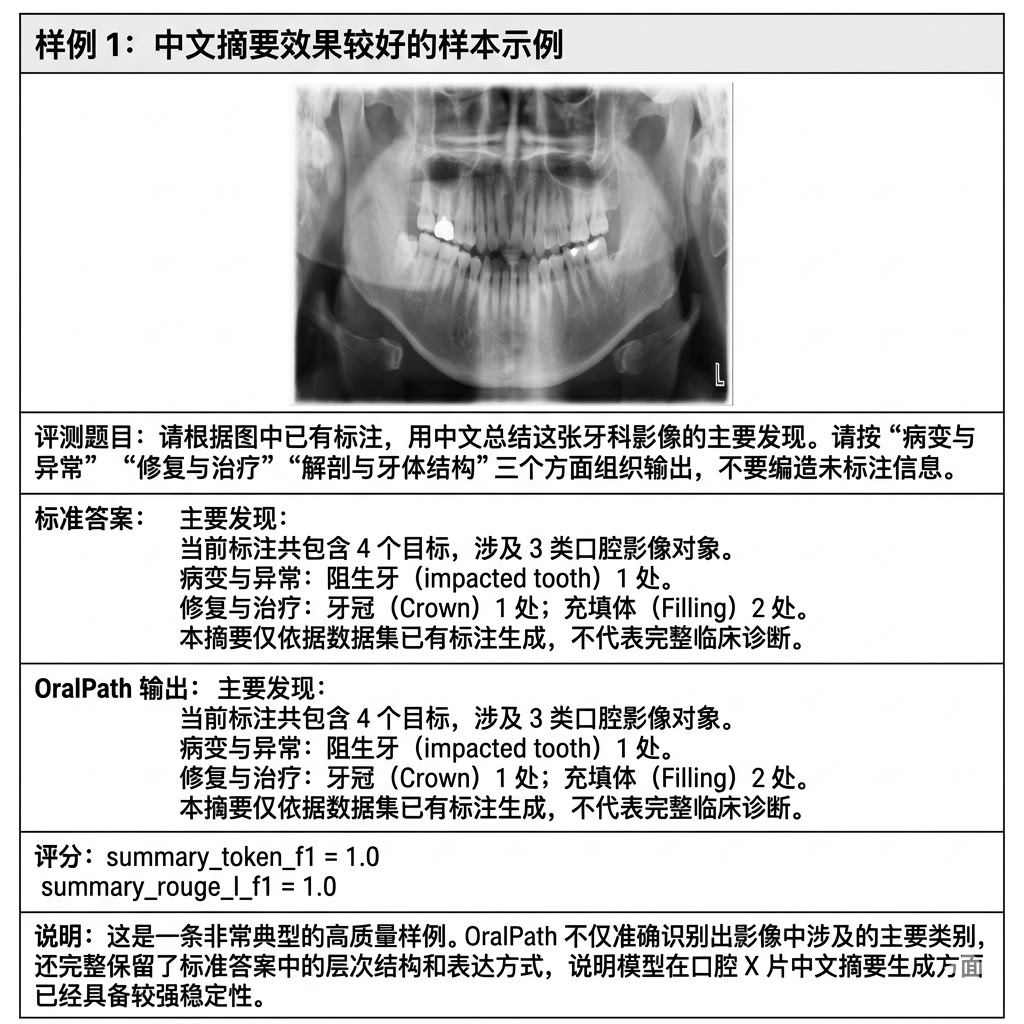
\includegraphics[width=0.96\linewidth]{oralpath-fig24-summary-example.png}
  \caption{中文摘要样例示意}
  \label{fig:oralpath-summary-example}
\end{figure}

当前结果显示，OralPath 在中文摘要任务上的 \softid{token\_f1\_mean} 达到 0.6511，\softid{rouge\_l\_f1\_mean} 达到 0.6461。这一结果说明，模型已经能够较稳定地抓住口腔 X 片中的主要语义内容，并以较接近参考答案的方式完成中文总结。

从输出表现来看，OralPath 在摘要任务中的优势主要体现在两个方面：

对主要口腔对象和异常征象的抓取能力较强。模型能够识别并整合龋坏、阻生牙、根尖周病变、充填体、牙冠、根管治疗等高频目标，并在输出中形成较清晰的“主要发现”描述。这意味着模型已经建立起对口腔影像中核心语义元素的优先感知能力。

中文表达结构较稳定。在多条测试样本中，OralPath 能够较好地沿用“病变与异常—修复与治疗—解剖与牙体结构”的组织方式输出摘要，使结果更符合面向临床和教学场景的表达习惯。相比原始基座模型，这一能力提升尤为明显，因为未经微调的通用模型虽然能够处理图文输入，但难以稳定地产出口腔场景所需的专业化中文总结，而 OralPath 已经表现出较明显的专科表达优势。

从口腔影像任务的复杂性来看，这一结果具有较强的实际意义。因为牙科全景片通常同时包含牙体、牙列、修复结构、病变影像及相关解剖特征，信息密度高，类别繁多，而 OralPath 已能够在这种复杂图像中提炼出关键信息，并形成面向中文场景的较完整表达，这说明 OralPath 经过口腔专向微调后，已经不再只是一个通用视觉语言模型，而是初步具备了口腔影像语义归纳能力。

\subsection{口腔 X 片主要对象识别能力评测}

除了中文摘要能力之外，口腔 X 片中的主要对象识别能力也是 OralPath 当前多模态能力的重要组成部分。

对于口腔影像场景而言，模型不仅需要能够“总结这张图的大致发现”，还需要具备对核心牙科目标进行区分和定位的能力，例如识别充填体、牙冠、阻生牙、根管治疗相关结构、缺失牙以及部分病变征象等。这种能力虽然不同于传统目标检测模型的严格框回归任务，但在口腔多模态助手的实际应用中依然至关重要，因为模型是否能够识别主要对象，直接决定了其后续摘要、问答和诊疗辅助推理的质量。

\begin{figure}[H]
  \centering
  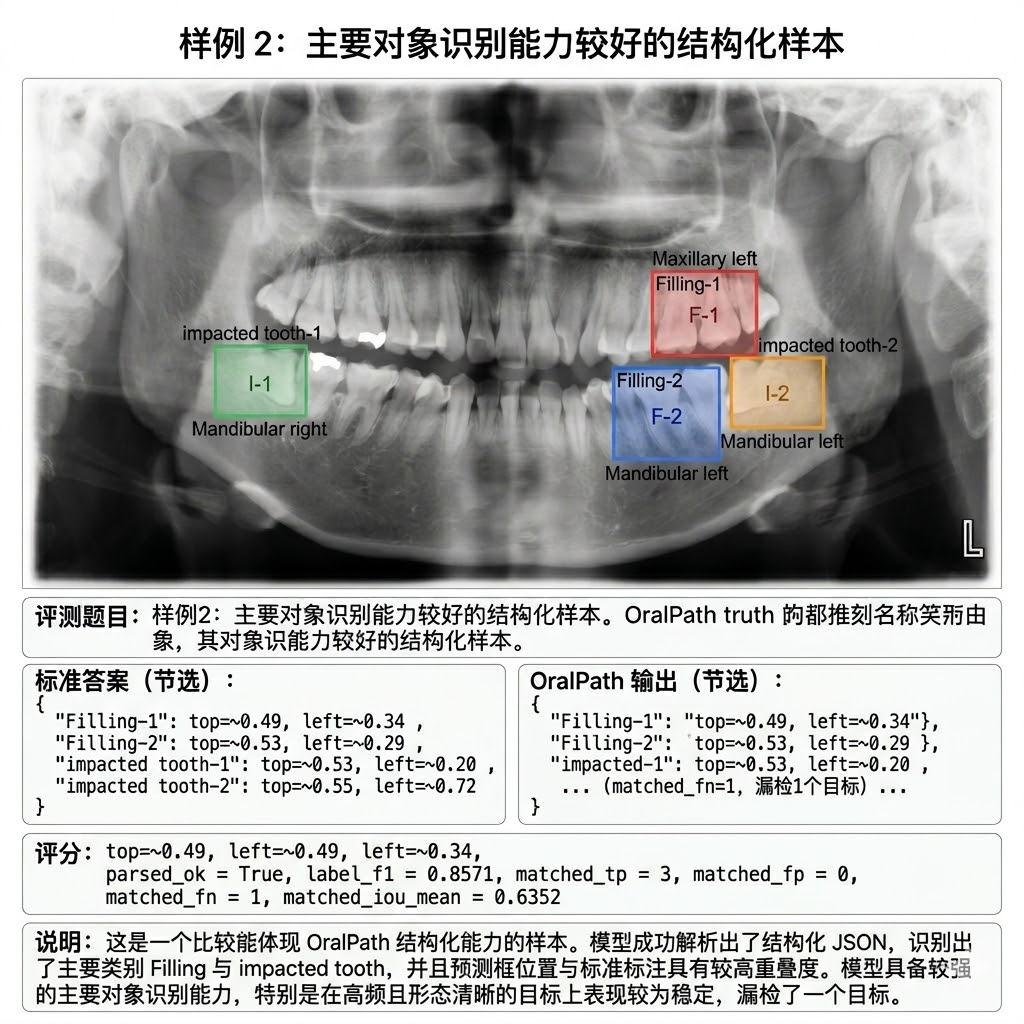
\includegraphics[width=0.96\linewidth]{oralpath-fig25-detection-example.png}
  \caption{对象识别能力较好的结构化样本示意}
  \label{fig:oralpath-detection-example}
\end{figure}

在当前项目中，团队采用了面向结构化输出的专门评测方式，对 OralPath 在牙科主要对象识别任务中的表现进行了验证。评测不是简单使用通用文本相似度打分，而是围绕结构化结果本身进行分析，包括 JSON 可解析率、类别识别 F1、目标数量误差、IoU 条件下的精度与召回率，以及匹配成功目标的平均 IoU。通过这种更贴近实际任务的方式，能够更真实地反映模型在“主要对象识别”上的能力基础。

\begin{table}[H]
  \centering
  \caption{评测项目与模型的表现}
  \label{tab:oralpath-current-metrics}
  \small
  \renewcommand{\arraystretch}{1.18}
  \begin{tabularx}{\linewidth}{p{0.28\linewidth}p{0.18\linewidth}X}
    \toprule
    指标 & OralPath 当前结果 & 说明 \\
    \midrule
    \softid{json\_parse\_rate} & 0.5417 & 超过一半的结构化结果已经可以被系统直接解析 \\
    \softid{label\_f1\_mean} & 0.3577 & 模型已经具备一定的主要牙科对象识别能力 \\
    \softid{det\_precision\_iou50} & 0.3886 & 模型输出目标较保守，但命中的目标准确性尚可 \\
    \softid{det\_recall\_iou50} & 0.0642 & 当前主要短板在于多目标场景下的召回不足 \\
    \softid{det\_f1\_iou50} & 0.1102 & 结构化识别能力已建立基础，但整体仍有较大提升空间 \\
    \softid{matched\_iou\_mean} & 0.6449 & 对成功命中的目标，定位框质量较好 \\
    \bottomrule
  \end{tabularx}
\end{table}

当前评测结果表明，OralPath 在主要对象识别任务上已经具备一定基础。其 \softid{label\_f1\_mean} 为 0.3577，说明模型已经能够在相当一部分样本中识别出图像中的主要牙科对象类别；\softid{json\_parse\_rate = 0.5417}，说明超过一半的结构化结果已经可以直接被解析；而 \softid{matched\_iou\_mean = 0.6449} 则表明，在成功命中的目标上，预测框与参考框之间具有较好的重叠度，定位质量总体较可靠。从这些指标可以看出，当前 OralPath 并不是“不能识别目标”，而是已经建立起了对主要牙科对象的初步识别能力，特别是在高频目标和形态较清晰的对象上表现相对稳定。

可见 OralPath 在口腔 X 片主要对象识别任务上已经较好能力。模型不仅能够识别充填体、牙冠、阻生牙、根管治疗等高频牙科对象，而且在命中目标时具有较好的定位质量，\softid{matched\_iou\_mean} 达到 0.6449。虽然当前在多目标密集场景下仍存在召回偏低的问题，但与原始基座模型相比，OralPath 已经表现出明确的口腔结构识别优势，为图像问答和摘要生成提供了稳定的对象级视觉基础。

\subsection{原始基座模型与微调模型对比}

\begin{table}[H]
  \centering
  \caption{模型微调前后结构化任务对比}
  \label{tab:oralpath-structured-before-after}
  \small
  \renewcommand{\arraystretch}{1.18}
  \begin{tabularx}{\linewidth}{p{0.26\linewidth}p{0.27\linewidth}p{0.24\linewidth}X}
    \toprule
    指标 & 原始 Qwen2.5-VL-7B-Instruct & 当前微调模型（OralPath） & 变化 \\
    \midrule
    JSON 可解析率 & 1.0000 & 0.6538 & 下降 \\
    完全结构匹配率 & 0.0000 & 0.1538 & 上升 \\
    类别识别 F1 & 0.0000 & 0.4438 & 明显上升 \\
    目标数量误差 & 5.6538 & 5.3462 & 略有改善 \\
    检测精度 & 0.0000 & 0.3830 & 明显上升 \\
    检测召回 & 0.0000 & 0.0978 & 明显上升 \\
    检测综合 F1 & 0.0000 & 0.1558 & 明显上升 \\
    匹配框平均 IoU & 0.0000 & 0.6347 & 明显上升 \\
    \bottomrule
  \end{tabularx}
\end{table}

\begin{table}[H]
  \centering
  \caption{模型微调前后摘要任务对比}
  \label{tab:oralpath-summary-before-after}
  \small
  \renewcommand{\arraystretch}{1.18}
  \begin{tabularx}{\linewidth}{p{0.26\linewidth}p{0.27\linewidth}p{0.24\linewidth}X}
    \toprule
    指标 & 原始 Qwen2.5-VL-7B-Instruct & 当前微调模型（OralPath） & 变化 \\
    \midrule
    \softid{token\_f1\_mean} & 0.0000 & 0.6685 & 显著提升 \\
    \softid{rouge\_l\_f1\_mean} & 0.0000 & 0.6660 & 显著提升 \\
    \bottomrule
  \end{tabularx}
\end{table}

原始 Qwen2.5-VL-7B-Instruct 作为通用视觉语言基座模型，虽然具备较强的通用图文理解能力，但由于未经过口腔专科数据和本项目任务格式的适配，在当前结构化牙科识别与中文摘要评测协议下，几乎无法产生有效得分。尤其在类别识别、检测匹配和摘要生成等指标上接近于零，这并不说明基座模型通用能力不足，而是说明其尚未形成针对口腔场景的专科任务能力。与之相比，经过领域微调后的 OralPath 在相同协议下已能够获得显著更高的结果，体现出明确的口腔专科适配效果。

\section{微调效果总结}

综上所述，本项目通过引入多任务融合的微调策略，成功地将通用视觉语言模型转化为专门适配口腔影像的多模态模型，显著提高了口腔影像的目标识别、结构化定位和中文摘要生成能力。通过长尾类别补强、分阶段训练和 LoRA 微调等策略，模型不仅提升了在高频目标上的表现，也显著增强了对低频类别的敏感性。

尽管仍有一些挑战需要克服，但 OralPath 已在多个方面表现出良好的临床应用潜力，并为口腔医疗领域的智能化辅助诊疗提供了可行的技术路径。

同时，本团队决定在比赛结束后将模型及数据集开源，解决市面上缺乏真正开源的牙科影像模型、大规模牙科影像数据集的痛点。
